% Created 2012-10-14 Sun 15:51
\documentclass[11pt]{article}
\usepackage[utf8]{inputenc}
\usepackage{fixltx2e}
\usepackage{url}
\usepackage{graphicx}
\usepackage{minted}
\usepackage{color}
\usepackage{longtable}
\usepackage{float}
\usepackage{wrapfig}
\usepackage{soul}
\usepackage{textcomp}
\usepackage{amsmath}
\usepackage{marvosym}
\usepackage{wasysym}
\usepackage{latexsym}
\usepackage{amssymb}
\usepackage[linktocpage,
  pdfstartview=FitH,
  colorlinks,
  linkcolor=blue,
  anchorcolor=blue,
  citecolor=blue,
  filecolor=blue,
  menucolor=blue,
  urlcolor=blue]{hyperref}
\usepackage{attachfile}
\tolerance=1000
\usepackage{adjustbox}
\usepackage{anysize}
\marginsize{1in}{1in}{1in}{1in}
\providecommand{\alert}[1]{\textbf{#1}}

\title{Molecular Simulation HOMEWORK 4}
\author{Zhongnan Xu}
\date{10/24/12 - Wednesday}
\hypersetup{
  pdfkeywords={},
  pdfsubject={},
  pdfcreator={Emacs Org-mode version 7.8.11}}

\begin{document}

\maketitle

\setcounter{tocdepth}{3}
\tableofcontents
\vspace*{1cm}


\section{Convergence study of tantalum}
\label{sec-1}
\subsection{Planewave cutoff convergence}
\label{sec-1-1}

Determine the planewave cutoff energy required to achieve a total energy convergence of 10 meV for bcc tantalum at its experimental lattice constant. Use a k-point grid of 10 \texttimes{} 10 \texttimes{} 10, and the PBE exchange correlation functional.


\begin{minted}[frame=lines,fontsize=\scriptsize,linenos]{python}
from ase import Atom, Atoms
from ase.visualize import view
from ase.lattice.cubic import BodyCenteredCubic
import numpy as np
import matplotlib.pyplot as plt
from jasp import *

# We will rely on the ase.lattice.cubic.BodyCenteredCubic module to give us
# the correct experimental lattice constant. Note we use the primitive cell
ready=True
Ta = BodyCenteredCubic('Ta', directions=[[-0.5, 0.5, 0.5],
                                         [0.5, -0.5, 0.5],
                                         [0.5, 0.5, -0.5]])
encuts = (150, 200, 250, 300, 350, 400, 450, 500, 550, 600)
energies = []
for cut in encuts:
    with jasp('1.1/e{0:d}'.format(cut),
              xc='PBE', lreal=False,
              encut=cut, prec='Accurate',
              kpts=(10, 10, 10), ismear=1, sigma=0.05,
              atoms=Ta) as calc:
        try:
            energies.append(Ta.get_potential_energy())
        except (VaspSubmitted, VaspQueued):
            energies.append(None)
            ready = False
            pass
assert len(encuts) == len(energies)
if not ready:
    import sys; sys.exit()

import matplotlib.pyplot as plt
from matplotlib.ticker import ScalarFormatter
# First offset the energies by the last value and find the absolute value
energies = np.array(energies)
energies -= energies[-1]*np.ones(len(energies))
energies = np.absolute(energies)
energies = energies*1000
fig = plt.figure(1, (5.5, 4.5))
ax = fig.add_subplot(111)
ax.plot(encuts, energies, label='Ta', marker='o')
ax.axhline(10, ls='--', label='10 meV Convergence')
ax.set_xlabel('Kinetic Energy Cutoff (eV)', size='large')
ax.set_ylabel('Total Energy (meV/atom)', size='large')
ax.legend(loc=0, prop={'size':'large'})
ax.yaxis.set_major_formatter(ScalarFormatter(useOffset=False))
fig.tight_layout()
plt.savefig('1-1.png')
plt.show()
\end{minted}


\begin{figure}[H]
\centering
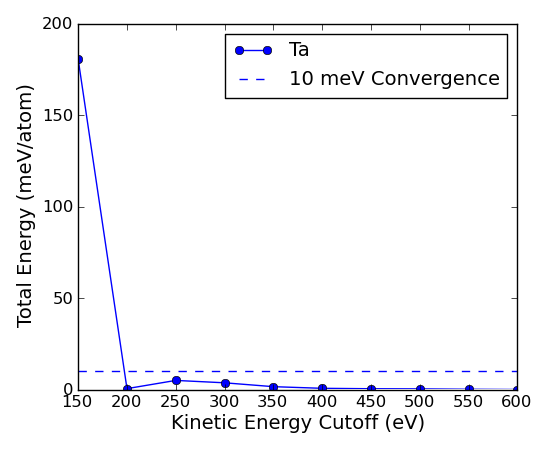
\includegraphics[width=0.7\textwidth]{./1-1.png}
\caption{Convergence of the total energy of BCC Ta at the experimental lattice cutoff}
\end{figure}

It is clear that the total energy of BCC Ta has already been converged at an energy cutoff of 200 eV. This should not be surprising considering the VASP site recommends a minimum cutoff of 220 eV.
\subsection{k-point grid convergence}
\label{sec-1-2}

Determine the Monkhorst-Pack k-point grid required to achieve a total energy convergence of 50 meV for bcc tantalum at its experimental lattice constant. Use a planewave cutoff of 350 eV for this study.


\begin{minted}[frame=lines,fontsize=\scriptsize,linenos]{python}
from ase import Atom, Atoms
from ase.visualize import view
from ase.lattice.cubic import BodyCenteredCubic
import numpy as np
import matplotlib.pyplot as plt
from jasp import *

# We will rely on the ase.lattice.cubic.BodyCenteredCubic module to give us
# the correct experimental lattice constant. Note we use the primitive cell
ready=True

Ta = BodyCenteredCubic('Ta', directions=[[-0.5, 0.5, 0.5],
                                         [0.5, -0.5, 0.5],
                                         [0.5, 0.5, -0.5]])
ks = (2, 4, 6, 8, 10, 12, 14, 16)
kpoints = []
for k in ks:
    kpoints.append((k, k, k))
energies = []
for kpoint in kpoints:
    with jasp('1.2/k{0:d}'.format(kpoint[0]),
              xc='PBE', lreal=False,
              encut=350, prec='Accurate',
              kpts=kpoint, ismear=1, sigma=0.05,
              atoms=Ta) as calc:
        try:
            energies.append(Ta.get_potential_energy())
        except (VaspSubmitted, VaspQueued):
            energies.append(None)
            ready = False
            pass
assert len(ks) == len(energies)
if not ready:
    import sys; sys.exit()

import matplotlib.pyplot as plt
from matplotlib.ticker import ScalarFormatter
# First offset the energies by the last value and find the absolute value
energies = np.array(energies)
energies -= energies[-1]*np.ones(len(energies))
energies = np.absolute(energies)
energies = energies*1000
fig = plt.figure(1, (5.5, 4.5))
ax = fig.add_subplot(111)
ax.plot(ks, energies, label='Ta', marker='o')
ax.axhline(50, ls='--', label='50 meV convergence')
ax.set_ylim((0, 100))
ax.set_xlabel(r'Kpoint Grid (N$\times$ N$\times$ N)', size='large')
ax.set_ylabel('Total Energy (meV/atom)', size='large')
ax.legend(loc=0, prop={'size':'large'})
ax.yaxis.set_major_formatter(ScalarFormatter(useOffset=False))
fig.tight_layout()
plt.savefig('1-2.png')
plt.show()
\end{minted}


\begin{figure}[H]
\centering
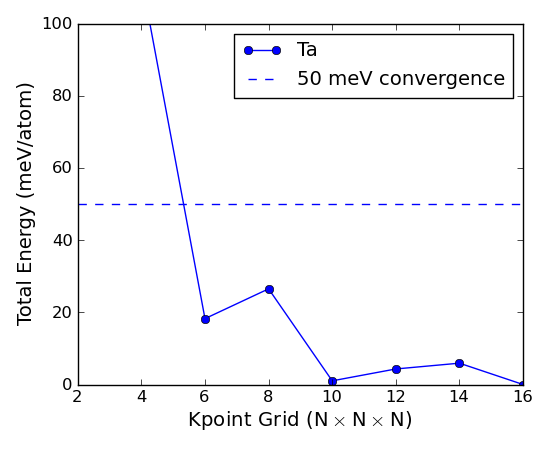
\includegraphics[width=0.7\textwidth]{./1-2.png}
\caption{Convergence of BCC Ta with respect to increasing k-point grid}
\end{figure}
\section{Convergence study of graphite}
\label{sec-2}
\subsection{Planewave convergence}
\label{sec-2-1}

Determine the planewave cutoff energy required to get convergence of 10 meV or better for graphite at its equilibrium lattice constant. Use a k-point grid of (6,6,6) for this study.
\subsection{k-point convergence}
\label{sec-2-2}

Determine the k-point grid required to get convergence of 50 meV or better for graphite at its equilibrium lattice constant. Use a planewave cutoff of 350 eV for this study.
\section{Determine the DFT lattice constant of bcc tantalum}
\label{sec-3}

Use the parameters you estimated in the previous problem. Construct an equation of state and determine the lattice constant and bulk modulus of tantalum. Compare your answers to literature values, and cite the source of your comparison.
\section{Determine the DFT lattice constant of fcc tantalum}
\label{sec-4}

Construct an equation of state to determine the lattice constant of fcc tantalum. You can assume the same parameters that were good for the bcc structure are good for the fcc structure. Which structure is more stable, fcc or bcc?
\section{Determine graphite lattice parameters}
\label{sec-5}

The crystal structure of graphite can be found at \href{http://cst-www.nrl.navy.mil/lattice/struk/a9.html}{http://cst-www.nrl.navy.mil/lattice/struk/a9.html} (or you can use the builtin \texttt{ase} functions).

Compute the geometry optimized total energy for graphite. Use parameters determined from the convergence study to ensure the total energy is converged to better than 50 meV. Compare your results to experimental data. Cite your source.
\section{Tantalum carbide lattice parameters}
\label{sec-6}

Tantalum carbide is a hard material. Use DFT to compute the lattice constant of cubic tantalum carbide in the rock salt structure (NaCl or B1), and the bulk modulus. The crystal structure of tantalum carbide can be found at \href{http://cst-www.nrl.navy.mil/lattice/struk/b1.html}{http://cst-www.nrl.navy.mil/lattice/struk/b1.html} or in the \texttt{ase.lattice} module. Compare the bulk modulus of the TaC to that of bcc tantalum. Which is harder?

The experimental lattice constant is 4.455 \AA{}, and the experimental bulk modulus is 3.45 Mbar. How do your results compare to this?
\section{Estimate the formation energy of TaC.}
\label{sec-7}

Compute the formation energy of TaC for the reaction Ta + C$_{\mathrm{graphite}}$ $\rightarrow$ TaC. Compare your anser to the value reported in \href{http://pubs.acs.org/doi/pdf/10.1021/j100786a027}{http://pubs.acs.org/doi/pdf/10.1021/j100786a027}. Discuss any reasons for discrepancy. Remember that you must use the same ENCUT for all the calculations in this problem, and you must use the largest ENCUT for all calculations that ensures the accuracy level you want.

\end{document}
